\chapter{Metodologia di semantic pruning}\label{chap:methodology}


\noindent Questo capitolo presenta la metodologia sviluppata. Le condizioni esatte di potatura,
derivate dal comportamento del sistema, costituiscono il criterio con cui le strategie vanno
lette: da esse discende che cosa si può rimuovere con garanzia e che cosa soltanto a costo di un
rischio dichiarato. Il capitolo motiva l'approccio, organizza lo spazio delle strategie lungo le
dimensioni che ne determinano la natura, descrive quelle implementate con il loro regime di
garanzia, la loro riduzione e il loro costo, spiega perché la generazione dei candidati non
ammetta una condizione esatta della stessa natura di quella che governa il veto, e definisce il
contratto con cui la potatura si integra nel sistema. Le proprietà formali e il risultato negativo
che delimita il campo di applicabilità sono oggetto del capitolo successivo.

% =======================================================================================
\section{Motivazioni}\label{sec:why-pruning}

Le ragioni per potare l'insieme delle RFD sono tre, di natura diversa, e la loro compresenza
spiega perché il problema non si riduca a un'ottimizzazione di prestazioni.

\paragraph{Ragione economica.} Il costo dell'imputazione cresce con il numero di regole: la
verifica dei veti esamina l'intero insieme per ogni imputazione candidata, e la
\autoref{sec:cost} mostra che è questa la voce dominante del tempo di esecuzione. Ridurre
l'insieme riduce quel costo, e la riduzione è tanto più preziosa quanto più il sistema è
impiegato su dataset di dimensioni maggiori.

\paragraph{Ragione di qualità.} Una regola non è necessariamente benefica. Regole con soglie
larghe competono nella generazione dei candidati e possono prevalere su regole più precise,
producendo imputazioni peggiori di quelle che si otterrebbero senza di esse. La potatura può
quindi migliorare il risultato, non soltanto accelerarlo: è la circostanza che il
\autoref{chap:results} misura, e che rende il problema interessante dal punto di vista della
qualità dei dati e non solo dell'efficienza.

\paragraph{Ragione epistemica.} Un insieme di migliaia di regole è esso stesso un oggetto
difficile da interpretare: non è ispezionabile, non è confrontabile fra dataset e non consente di
attribuire un comportamento a una causa. La selezione di un sottoinsieme rilevante ha valore
conoscitivo indipendentemente dal guadagno prestazionale, perché è la condizione per cui il
comportamento del sistema diventa spiegabile.

\paragraph{La tensione che governa il problema.} Le tre ragioni convergono su un'unica
operazione --- rimuovere regole --- ma il sistema studiato assegna a ogni regola due ruoli
distinti, la generazione dei candidati e il veto sulle imputazioni incoerenti, governati da
requisiti opposti sulla stessa grandezza: una soglia stretta rende la regola più selettiva come
generatore e più severa come veto, mentre una soglia larga la rende più permissiva come generatore
e più debole come veto. Nulla, nel formato del file, distingue i due ruoli
(\autoref{sec:dual-role}). Ne segue che ogni strategia di rimozione deve dichiarare
\emph{quale} dei due ruoli è disposta a sacrificare, e che la nozione di ``potatura sicura''
(\autoref{def:safe-pruning}) richiede di specificare rispetto a che cosa la sicurezza è pretesa.
È questa precisazione a rendere possibile il risultato negativo del \autoref{chap:theory}.

% =======================================================================================
\section{Dal sistema alle condizioni esatte}\label{sec:exact-conditions}

\begin{algorithm}[htbp]
\caption{Ricerca dei copritori per la condizione \Vtwo{}. Il parametro $\mu$ limita la differenza
di ampiezza fra il lato sinistro della regola coprente e quello della regola coperta; la
\autoref{sec:maxextra} mostra che il risultato non dipende dal suo valore.}
\label{alg:cover}
\begin{algorithmic}[1]
\State \textbf{input}: insieme di regole $R$, dataset $D$, parametro $\mu$
\State $C \gets \emptyset$ \Comment{regole la cui rimozione è garantita}
\ForAll{$r \in R$ con $\LHS(r) \cap \NullCols(D) \neq \emptyset$}
    \ForAll{$r'' \in R \setminus \{r\}$ con $\RHS(r'') = \RHS(r)$ e
            $|\LHS(r)| - |\LHS(r'')| \le \mu$}
        \If{$\LHS(r'') \subseteq \LHS(r)$ \textbf{and} $\theta_{r''}(c) \ge \theta_r(c)\ \forall c \in \LHS(r'')$
            \textbf{and} $\theta_{\RHS}(r'') \le \theta_{\RHS}(r)$}
            \State $C \gets C \cup \{r\}$ \Comment{$r''$ copre $r$}
            \State \textbf{break}
        \EndIf
    \EndFor
\EndFor
\State \Return $C$
\end{algorithmic}
\end{algorithm}

Le condizioni che seguono non sono ipotizzate a priori: sono ricavate dal comportamento effettivo
del sistema, letto sul bytecode decompilato, e classificate in base al ruolo che una regola
\emph{può} svolgere. Esse costituiscono il fondamento della metodologia e la base del risultato
negativo del \autoref{chap:theory}.

\begin{definition}[Condizione \Vone{} --- veto impossibile]\label{def:v1}
Sia $\NullCols$ l'insieme delle colonne del dataset che presentano almeno una cella nulla. Una
RFD $r$ \emph{non può} esercitare alcun veto se
\[
    \LHS(r) \cap \NullCols = \emptyset .
\]
\end{definition}

La condizione è necessaria e sufficiente: la verifica di coerenza confronta valori, e il confronto
richiede che entrambi i valori siano presenti. Se nessuna colonna del lato sinistro presenta
valori mancanti, la verifica non può essere attivata.

\begin{definition}[Condizione \Vtwo{} --- veto coperto]\label{def:v2}
Una RFD $r$ è \emph{coperta} se esiste una RFD $r''$ tale che:
\begin{enumerate}[label=(\roman*),leftmargin=1.8em]
    \item $\RHS(r'') = \RHS(r)$ e $\LHS(r'') \subseteq \LHS(r)$, con $\LHS(r'') \neq \emptyset$;
    \item $\theta_{r''}(c) \ge \theta_r(c)$ per ogni $c \in \LHS(r'')$ (soglie \emph{più larghe});
    \item $\theta_{\RHS}(r'') \le \theta_{\RHS}(r)$ (soglia di destra \emph{più stretta}).
\end{enumerate}
\end{definition}

\begin{proposition}[Correttezza di \Vtwo{}]\label{prop:v2}
Se $r''$ copre $r$ secondo la Definizione~\ref{def:v2} e $r''$ sopravvive alla potatura, allora ogni veto
esercitato da $r$ è implicato da un veto di $r''$.
\end{proposition}

\begin{proof}
Sia $t$ una tupla che attiva il veto di $r$. Per definizione esistono una tupla $s$ e una colonna
$c \in \LHS(r)$ tali che $s$ e $t$ concordano entro $\theta_r(c)$ su $c$, e $s$ e $t$ differiscono
su $\RHS(r)$ di più di $\theta_{\RHS}(r)$.

Poiché $\LHS(r'') \subseteq \LHS(r)$, la tupla $s$ concorda con $t$ anche su ogni colonna di
$\LHS(r'')$: per la condizione (ii) le soglie di $r''$ sono più larghe, dunque l'accordo entro
$\theta_r(c)$ implica l'accordo entro $\theta_{r''}(c)$. La condizione (i) garantisce che
$\LHS(r'')$ non sia vuoto, sicché la verifica di $r''$ ha almeno una colonna su cui essere
valutata. Infine, per la condizione (iii), la differenza su $\RHS$ che supera $\theta_{\RHS}(r)$
supera a maggior ragione $\theta_{\RHS}(r'')$. Dunque $s$ e $t$ attivano anche il veto di $r''$.
\end{proof}

\begin{remark}
La direzione delle disuguaglianze è controintuitiva rispetto alla nozione classica di dominanza
fra dipendenze, dove si è soliti richiedere che la regola dominante sia \emph{più stretta}. Qui
occorre l'opposto: la regola coprente deve essere più permissiva sul lato sinistro e più severa
su quello destro, perché è la severità sul destro a implicare il rifiuto.
\end{remark}

\begin{definition}[Condizione \Vthree{} --- regola inerte]\label{def:v3}
Una RFD $r$ è \emph{provabilmente inerte} se
\[
    \LHS(r) \cap \NullCols = \emptyset \quad \wedge \quad \RHS(r) \notin \NullCols .
\]
\end{definition}

Una regola inerte non può né generare candidati --- la colonna di destra non ha celle nulle --- né
esercitare veti --- per la \Vone{}. La sua rimozione è quindi priva di effetti per costruzione.

\begin{table}[htbp]
\centering
\caption{Dimensione delle tre classi. Le classi \Vtwo{} e \Vthree{} sono disgiunte sui dati
esaminati: la loro unione è quindi la riduzione massima ottenibile con le condizioni esatte.}
\label{tab:conditions}
\footnotesize
\begin{tabular}{llrrrrr}
\toprule
famiglia & soglia & $N$ & \Vthree{} inerte & \Vtwo{} coperta & unione \\
\midrule
Bridges    & 3  & \num{1830}  & 2 (\SI{0.11}{\percent}) & 215  & \SI{11.9}{\percent} \\
Bridges    & 9  & \num{8961}  & 6 (\SI{0.07}{\percent}) & \num{1531} & \SI{17.2}{\percent} \\
Bridges    & 15 & \num{18844} & 6 (\SI{0.03}{\percent}) & \num{3927} & \SI{20.9}{\percent} \\
Glass      & 3  & \num{1511}  & 5 (\SI{0.33}{\percent}) & 40   & \SI{3.0}{\percent} \\
Glass      & 9  & \num{11648} & 18 (\SI{0.15}{\percent}) & 861 & \SI{7.5}{\percent} \\
Glass      & 15 & \num{27445} & 24 (\SI{0.09}{\percent}) & \num{2363} & \SI{8.7}{\percent} \\
Restaurant & 3  & 25          & 0 & 0   & \SI{0.0}{\percent} \\
Restaurant & 6  & 124         & 0 & 2   & \SI{1.6}{\percent} \\
\bottomrule
\end{tabular}
\end{table}

La \autoref{tab:conditions} mostra due fatti che orientano il resto del lavoro. Il primo è che la
classe \Vthree{} è trascurabile su tutte le famiglie, non soltanto su Bridges: la ragione è
strutturale, poiché richiede regole il cui lato sinistro impieghi esclusivamente colonne mai
nulle, e tali colonne sono poche. Il secondo è che la classe \Vtwo{} è l'unica leva
significativa, e cresce con la soglia fino a poco più di un quinto dell'insieme.

% =======================================================================================
\section{Lo spazio delle strategie}\label{sec:strategy-space}

\begin{figure}[htbp]
\centering
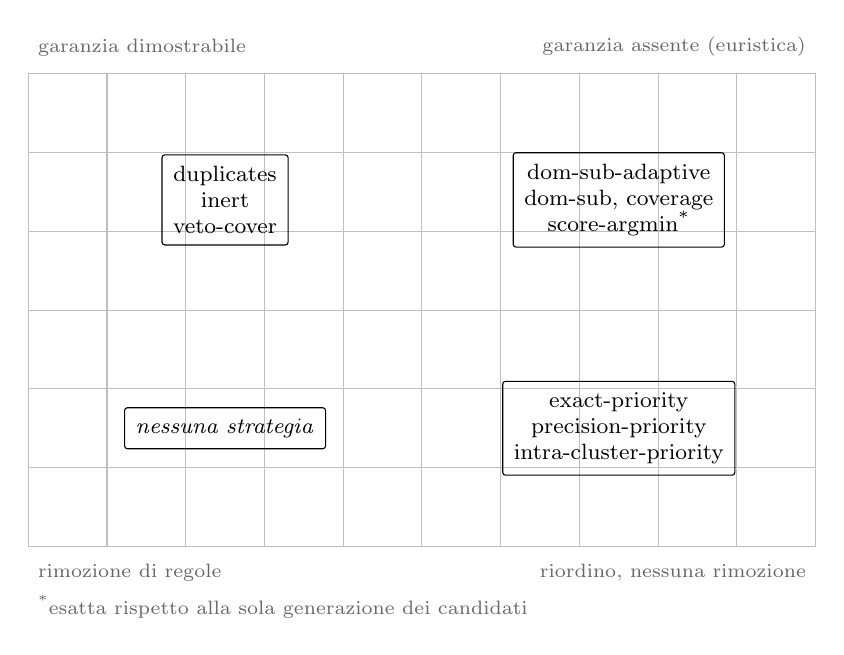
\begin{tikzpicture}[font=\footnotesize, every node/.style={align=center}]
\draw[black!25] (0,0) grid (10,6);
\node[anchor=south west, font=\scriptsize, black!60] at (0,6.1) {garanzia dimostrabile};
\node[anchor=south east, font=\scriptsize, black!60] at (10,6.1) {garanzia assente (euristica)};
\node[anchor=north west, font=\scriptsize, black!60] at (0,-0.1) {rimozione di regole};
\node[anchor=north east, font=\scriptsize, black!60] at (10,-0.1) {riordino, nessuna rimozione};
\node[draw, rounded corners=1pt, inner sep=4pt] at (2.5,4.4) {\str{duplicates}\\ \str{inert}\\ \str{veto-cover}};
\node[draw, rounded corners=1pt, inner sep=4pt] at (7.5,4.4) {\str{dom-sub-adaptive}\\ \str{dom-sub}, \str{coverage}\\ \str{score-argmin}\textsuperscript{*}};
\node[draw, rounded corners=1pt, inner sep=4pt] at (2.5,1.5) {\emph{nessuna strategia}};
\node[draw, rounded corners=1pt, inner sep=4pt] at (7.5,1.5) {\str{exact-priority}\\ \str{precision-priority}\\ \str{intra-cluster-priority}};
\node[anchor=north west, font=\scriptsize, black!60] at (0,-0.5) {\textsuperscript{*}esatta rispetto alla sola generazione dei candidati};
\end{tikzpicture}
\caption{Collocazione delle strategie rispetto a che cosa modificano e a che cosa garantiscono.
Il quadrante in basso a sinistra è vuoto per costruzione: una strategia che non rimuove regole non
ha bisogno di garanzie, e una che le rimuove senza garanzia appartiene al quadrante in alto a
destra.}
\label{fig:taxonomy}
\end{figure}

Le diciannove strategie implementate non sono un elenco di tentativi: si distribuiscono lungo tre
dimensioni indipendenti, che ne determinano la natura e le possibilità.

\begin{description}[leftmargin=1.4em]
    \item[Che cosa cambiano.] Le strategie di \emph{rimozione} riscrivono il file eliminando
    regole; le strategie di \emph{riordino} non eliminano nulla e modificano soltanto la posizione
    delle righe. La distinzione non è di intensità ma di natura: il riordino è l'unica classe che
    preserva entrambi i ruoli per costruzione, perché nessuna regola viene sottratta al sistema, e
    il suo effetto è quindi interamente mediato dal comportamento dell'algoritmo.
    \item[Che cosa garantiscono.] Una strategia è \emph{esatta} se la sua applicazione è
    dimostrabilmente priva di effetti --- la rimozione è giustificata da una proprietà che si
    verifica sul file delle regole e sullo schema dei valori mancanti --- ed \emph{euristica} se
    la rimozione è plausibile ma non garantita. La distinzione è mantenuta in ogni fase: nelle
    strategie, nella politica di tutela dei veti e nella presentazione dei risultati.
    \item[Che informazione richiedono.] Alcune strategie decidono guardando soltanto il file delle
    regole; altre richiedono un'analisi del dataset (il calcolo statico dell'argomento del minimo,
    la stima della copertura empirica). Il costo di questa analisi è un costo di preprocessing, che
    va confrontato con il risparmio ottenuto in esecuzione: la \autoref{sec:cost} mostra che il
    confronto non è sempre favorevole.
\end{description}

Dalla combinazione delle tre dimensioni discende il criterio con cui le strategie sono presentate
nel seguito: per ciascuna si dichiarano la famiglia, il regime di garanzia, l'informazione
richiesta, la riduzione osservata e l'effetto misurato sulla qualità. Le strategie che non
soddisfano il criterio di garanzia non sono presentate come alternative equivalenti ma come
strumenti con un profilo di rischio esplicito.

% =======================================================================================
% =======================================================================================
\section{Le strategie di potatura}\label{sec:strategies}

\begin{algorithm}[htbp]
\caption{Driver di potatura. Le rimozioni garantite sono esenti dal computo del budget: essendo
prive di costo in termini di veto, addebitarle costituirebbe una doppia contabilizzazione.}
\label{alg:driver}
\begin{algorithmic}[1]
\State \textbf{input}: regole $R$, dataset $D$, strategia $S$, politica $\pi$, frazione $F$
\State $R' \gets S(R, D)$ \Comment{trasformazione richiesta dalla strategia}
\State $G \gets \{ r \in R \setminus R' : r \in C \ \textbf{or}\ r \in I \}$
       \Comment{rimozioni garantite: $C$ da \Vtwo{}, $I$ da \Vthree{}}
\State $H \gets \{ r \in R \setminus (R' \cup G) : \LHS(r) \cap \NullCols(D) \neq \emptyset \}$
       \Comment{rimozioni che sacrificano un veto}
\If{$\pi = \str{protect}$}
    \State $H \gets \emptyset$
\ElsIf{$\pi = \str{budget:F}$}
    \State ordina $H$ per indice di rischio crescente
    \State $H \gets$ le $\lceil F \cdot |H| \rceil$ regole di $H$ a rischio minore
           \Comment{le altre sono ripristinate}
\EndIf
\State \textbf{output}: $R \setminus (G \cup H)$
\end{algorithmic}
\end{algorithm}

La \autoref{tab:strategies} riassume le strategie principali, con la garanzia associata, la
riduzione osservata e l'effetto misurato sulla qualità\footnote{Le riduzioni e gli effetti
provengono da esperimenti diversi, indicati nella colonna ``effetto'' e descritti nel
\autoref{chap:experiments}: l'ablazione impiega venti configurazioni comuni su Bridges,
l'esperimento di ordinamento quindici configurazioni alla soglia 9, la campagna principale le
cinquanta configurazioni di Bridges. I valori non sono quindi confrontabili fra righe diverse
della tabella.}.

\begin{table}[htbp]
\centering
\caption{Strategie di potatura implementate. ``Garanzia'' indica se la rimozione è dimostrabilmente
priva di effetti; ``riduzione'' è l'ordine di grandezza osservato sui dataset impiegati;
``effetto'' è la variazione di imputazioni corrette rispetto alla configurazione non potata,
misurata nell'esperimento indicato. Le strategie citate nel seguito del lavoro sono in grassetto.}
\label{tab:strategies}
\footnotesize
\begin{tabular}{@{}llccp{2.9cm}@{}}
\toprule
famiglia & strategia & garanzia & riduzione & effetto misurato \\
\midrule
\multirow{3}{*}{strutturale}
  & \str{duplicates}        & sì & \SI{0}{\percent} & nessuno \\
  & \str{veto-dominance}    & no  & --- & non impiegata \\
  & \str{dom-exact}         & no  & --- & non impiegata \\
\midrule
\multirow{3}{*}{esatta}
  & \textbf{\str{veto-cover}}      & \textbf{sì} & \SI{0}{\percent}--\SI{20.9}{\percent} & nessuno (\num{113}/\num{113} configurazioni identiche) \\
  & \str{inert}             & sì & \SI{0.03}{\percent}--\SI{0.33}{\percent} & nessuno, per costruzione \\
  & \str{score-argmin}      & sì\textsuperscript{*} & fino a \SI{98}{\percent}\textsuperscript{*} & nessuna perdita di copertura, ma rallentamento fino a \num{251}$\times$ \\
\midrule
\multirow{4}{*}{euristica}
  & \textbf{\str{dom-sub-adaptive}} & no & \SI{32}{\percent}--\SI{93}{\percent} & $-20$ corrette da sola (ablazione) \\
  & \str{dom-sub}, \str{dom-sub-strict} & no & \SI{67}{\percent}--\SI{90}{\percent} & non impiegate da sole \\
  & \str{used}, \str{empirical}     & no & variabile & non impiegate da sole \\
  & \str{coverage}, \str{lhs-cap}, \str{rhs-thr} & no & variabile & non impiegate da sole \\
\midrule
\multirow{3}{*}{di riordino}
  & \textbf{\str{exact-priority}}   & no & \SI{0}{\percent} & $+25$ corrette da solo (ablazione) \\
  & \textbf{\str{precision-priority}} & no & \SI{0}{\percent} & $+53$ corrette (ordinamento) \\
  & \str{intra-cluster-priority}    & no & \SI{0}{\percent} & nessuno (\num{15}/\num{15} configurazioni identiche) \\
\bottomrule
\end{tabular}

\vspace{0.4em}
\raggedright\footnotesize\textsuperscript{*}La garanzia di \str{score-argmin} riguarda la sola
generazione dei candidati, non il potere di veto: la precisazione è essenziale ed è discussa nel
\autoref{sec:score-argmin}.
\end{table}

\paragraph{La strategia garantita: \str{veto-cover}.} Elimina le regole il cui veto è implicato da
una regola sopravvissuta, secondo la condizione \Vtwo{} della \autoref{sec:exact-conditions}. È
l'unica strategia di rimozione che offra una garanzia dimostrabile su entrambi i ruoli, e la sua
riduzione è per questo limitata: cresce con la soglia e non supera il \SI{20.9}{\percent} sui
dataset esaminati. La \autoref{sec:res-vetocover} ne verifica l'equivalenza di output.

\paragraph{Le strategie esatte di portata limitata.} \str{inert} rimuove le regole inerti secondo
la condizione \Vthree{}: la garanzia è totale e la riduzione trascurabile, circostanza che
costituisce di per sé un risultato negativo sulla praticabilità di questa via.
\str{score-argmin} preserva la generazione calcolando staticamente, per ogni cella nulla,
l'argomento del minimo che il sistema sceglierebbe: può rimuovere fino al \SI{98}{\percent} delle
regole, ma non preserva il veto, e la \autoref{sec:negative-results} mostra che il suo effetto sul
tempo è opposto a quello atteso.

\paragraph{Le strategie euristiche.} \str{dom-sub-adaptive} rimuove regole che risultano dominate
rispetto a una relazione di sussunzione adattata ai dati, con una soglia di aggressività
regolabile. È la strategia che produce le riduzioni maggiori, ed è anche quella il cui effetto
sulla qualità dipende dal dataset: la combinazione impiegata nelle campagne principali
(\str{A5b}) la associa al riordino per priorità di precisione.

\paragraph{Le strategie di riordino.} Non eliminano regole e non sono soggette ad alcuna politica
di tutela. \str{exact-priority} dispone per prime le regole che producono il valore esatto,
\str{precision-priority} quelle con la precisione empirica più alta, \str{intra-cluster-priority}
interviene sull'ordine interno ai cluster. Il loro effetto è mediato dalle due procedure di
riempimento (\autoref{sec:two-branches}) ed è oggetto dell'esperimento di ordinamento
i cui esiti sono riportati nella \autoref{sec:negative-results}.

\paragraph{Componibilità delle strategie.} Le famiglie non sono intercambiabili e la loro
composizione non è libera. Il \emph{riordino} si compone con qualunque strategia di rimozione,
perché non sottrae regole e non consuma budget di veto; la \emph{rimozione garantita} si compone
con l'euristica, ma il suo effetto si somma a quello dell'euristica soltanto se le due agiscono su
regole diverse. \str{score-argmin} non si compone con le altre strategie di rimozione: la sua
garanzia riguarda la generazione e vale rispetto all'insieme di partenza, sicché una rimozione
successiva può invalidare l'argomento del minimo che essa ha calcolato staticamente. È la ragione
per cui la combinazione impiegata nelle campagne è formata da un riordino e da una sola strategia
di rimozione euristica, e non da più rimozioni in cascata.

\section{Perché la generazione non ammette una condizione esatta della stessa natura}
\label{sec:generation-limit}

La condizione \Vtwo{} sfrutta una proprietà logica del veto: se una regola ne implica un'altra, la
seconda è superflua. Per la generazione una proprietà analoga non sussiste, e la ragione è
strutturale: il valore imputato dipende dal \emph{miglior punteggio} fra i candidati di un cluster,
e il miglior punteggio dipende dall'insieme delle regole presenti. Rimuovere una regola può quindi
cambiare l'argomento del minimo anche quando quella regola non è mai essa stessa il minimo. La
generazione è perciò una funzione dell'\emph{insieme}, non un insieme di contributi indipendenti,
e nessuna proprietà locale di una singola regola può certificare che la sua assenza non alteri
l'esito.

Da qui la distinzione fra la condizione \str{score-argmin}, che preserva la generazione
\emph{calcolando} staticamente l'argomento del minimo sul dataset --- quindi pagando un costo di
preprocessing proporzionale alla dimensione dei dati --- e le strategie euristiche, che rinunciano
a questa proprietà in cambio di riduzioni maggiori. La stessa asimmetria fra i due ruoli è la
ragione per cui, come dimostra il \autoref{chap:theory}, una potatura che operi sul solo file
delle regole non possa superare la classe delle regole coperte e delle regole inerti senza
rinunciare a una garanzia.

% =======================================================================================
\section{Integrazione con il sistema: il contratto di potatura}\label{sec:integration}

\paragraph{Preprocessing esterno.} La potatura si inserisce fra l'estrazione delle RFD e
l'esecuzione del sistema: il file delle regole viene riscritto secondo la strategia scelta, e il
sistema viene eseguito sul file risultante. Il dataset non è modificato, e l'eseguibile non è
toccato. La scelta ha il pregio di non richiedere alcuna modifica al sistema --- che resta quello
originale, verificato per checksum --- ed è stata mantenuta come vincolo per l'intera durata del
lavoro; la \autoref{sec:instrumentation} mostra che il vincolo è stato rimosso per una parte
dell'analisi, ma le strategie di potatura operano tutte nella forma esterna.

\paragraph{Politica sui veti.}\label{sec:veto-policy}
Poiché la rimozione di una regola può sacrificarne il potere di veto, ogni strategia di rimozione
è accompagnata da una politica esplicita, scelta fra tre:

\begin{itemize}[leftmargin=1.4em]
    \item \str{protect}: ogni regola in grado di esercitare un veto viene ripristinata. La
    riduzione si annulla, ma la garanzia è totale;
    \item \str{budget:F}: è consentito rimuovere una frazione $F$ delle regole portatrici di veto,
    scelte secondo un ordinamento di rischio;
    \item \str{allow}: nessuna tutela. La riduzione è massima e il potere di veto è
    esplicitamente sacrificato.
\end{itemize}

Le rimozioni il cui veto è \emph{provato coperto} dalla condizione \Vtwo{} sono esenti dal
computo del budget: essendo prive di costo in termini di veto, addebitarle costituirebbe una
doppia contabilizzazione. Questa precisazione, insieme a un difetto di correttezza della prima
implementazione, è discussa nel \autoref{chap:defects}.

\paragraph{Invarianti del contratto.} Il contratto di potatura è soggetto a tre invarianti,
verificate automaticamente dall'ambiente di valutazione. Il file prodotto deve essere un
sottoinsieme del file di partenza con lo stesso formato, e il dataset non deve essere alterato; le
righe devono conservare contenuto e ordinamento relativo, così che una strategia di riordino sia
distinguibile da una di rimozione; se il file prodotto coincide con quello di partenza, il
confronto è \emph{vacuo} e va segnalato anziché conteggiato come esito nullo. La terza invariante
è quella che nella pratica si è rivelata più utile, perché un numero non trascurabile di
configurazioni produce una potatura vuota, e trattarle come evidenza di assenza di effetto
avrebbe alterato le conclusioni.
